\eqref{eq:solutions/2/6/24/eq:1.1} can also be written as 
\begin{equation}\label{eq:solutions/2/6/24/eq:2.1}
\vec{x}^T \myvec{a && b \\ b && c} \vec{x} + \myvec{d && e}\vec{x} + f = 0
\end{equation}
\begin{equation}\label{eq:solutions/2/6/24/eq:2.2}
\begin{split}
\vec{V}=\myvec{6 && k/2\\ k/2 && -3}\\
\vec{u}=\myvec{2\\5/2}\\
f= -2
\end{split}
\end{equation}
Block Matrix
\begin{equation} \label{eq:solutions/2/6/24/eq:2.3}
 = \myvec{6 && k/2 && 2\\ k/2 && -3 && 5/2\\2 && 5/2 && -2}
\end{equation} 
Determinant of the Block Matrix
\begin{equation} \label{eq:solutions/2/6/24/eq:2.4}
\Delta = \mydet{6 && k/2 && 2\\ k/2 && -3 && 5/2\\2 && 5/2 && -2}
\end{equation}
If the \eqref{eq:solutions/2/6/24/eq:1.1} represents a pair of straight lines\\
then the Determinant is zero
\begin{equation} \label{eq:solutions/2/6/24/eq:2.5}
\begin{split}
\Delta = 0\\
\implies \mydet{6 && k/2 && 2\\ k/2 && -3 && 5/2\\2 && 5/2 && -2} = 0\\
\implies 6\times(6-25/4)-k/2(-k-5)+2(5k/4+6) = 0\\
\implies k^2 + 10k + 21 = 0
\end{split}
\end{equation}
\begin{equation} \label{eq:solutions/2/6/24/eq:2.6}
\begin{split} 
\implies \boxed{ k = -3 }\\
\implies \boxed{ k = -7 }
\end{split}
\end{equation}
Substituting k=-3 in \eqref{eq:solutions/2/6/24/eq:1.1}
\begin{equation} \label{eq:solutions/2/6/24/eq:2.7}
\vec{x}^T \myvec{6 && -3/2 \\ -3/2 && -3} \vec{x} + \myvec{4 && 5}\vec{x} -2 = 0
\end{equation}
\eqref{eq:solutions/2/6/24/eq:2.2} can be represented as 
\begin{equation} \label{eq:solutions/2/6/24/eq:2.8}
\begin{split}
\vec{V}=\myvec{6 && -3/2\\ -3/2 && -3}\\
\vec{u}=\myvec{2\\5/2}\\
f= -2
\end{split}
\end{equation}
To find the separate equations of the straight lines we will use spectral decomposition.\\
Characteristic equation of $\vec{V}$ is given by:
\begin{equation} \label{eq:solutions/2/6/24/eq:2.9}
\begin{split}
\mydet{V-\lambda \vec{I}}=\mydet{6-\lambda && -3/2\\ -3/2 && -3-\lambda} = 0\\
\implies \lambda^2 - 3\lambda - 81/4 = 0
\end{split}
\end{equation}
The Eigen Values of $\vec{V}$ are:
\begin{equation} \label{eq:solutions/2/6/24/eq:2.10}
\lambda_1 = \frac{3+3\sqrt{10}}{2}, \lambda_2 = \frac{3-3\sqrt{10}}{2}
\end{equation}
Let $\vec{p}_1$ and $\vec{p}_2$ be the Eigen vector corresponding to $\lambda_1$ and $\lambda_2$ respectively\\
Eigen vector $\vec{p}$ is given as:
\begin{equation} \label{eq:solutions/2/6/24/eq:2.11}
\begin{split}
\vec{V}\vec{p} = \lambda\vec{p}\\
\implies (\vec{V} - \lambda \vec{I})\vec{p} = 0
\end{split}
\end{equation}
For $\lambda_1 = \frac{3+3\sqrt{10}}{2}$
\begin{equation}\label{eq:solutions/2/6/24/eq:2.12}
(\vec{V} - \lambda_1 \vec{I}) = \myvec{\frac{9-3\sqrt{10}}{2} && -3/2\\ -3/2 && \frac{-9-3\sqrt{10}}{2}}
\end{equation}
To find $ \vec{p}_1 $ Use Augmented Matrix of $(\vec{V} - \lambda \vec{I})$
\begin{equation} \label{eq:solutions/2/6/24/eq:2.13}
\begin{split}
 \myvec{\frac{9-3\sqrt{10}}{2} && -3/2 && 0\\ -3/2 && \frac{-9-3\sqrt{10}}{2} && 0}\\
\xleftrightarrow[]{R_1\rightarrow \frac{2}{9-3\sqrt{10}}R_1} 
\myvec{1 && 3+\sqrt{10} && 0\\ -3/2 && \frac{-9-3\sqrt{10}}{2} && 0}\\
\xleftrightarrow[]{R_1\rightarrow 3/2R_1+R_2} 
\myvec{1 && 3+\sqrt{10} && 0\\ 0 && 0 && 0} 
\end{split}
\end{equation}
So we get,
\begin{equation}\label{eq:solutions/2/6/24/eq:2.14}
x_1 + (3+\sqrt{10})x_2 = 0
\end{equation}
Therefore, Eigen Vector corresponding to $\lambda_1$
\begin{equation}\label{eq:solutions/2/6/24/eq:2.15}
\vec{p}_1 =\frac{1}{\sqrt{20+6\sqrt{10}}} \myvec{-(3+\sqrt{10}) \\ 1}
\end{equation}
Similarly for $\lambda_2 = \frac{3-3\sqrt{10}}{2}$
\begin{equation}\label{eq:solutions/2/6/24/eq:2.16}
\vec{p}_2 =\frac{1}{\sqrt{20-6\sqrt{10}}} \myvec{-(3-\sqrt{10}) \\ 1}
\end{equation}
We know that $\vec{V} = \vec{P}\vec{D}\vec{P}^T$ where $\vec{P}$ and $\vec{V}$ are given by:
\begin{equation} \label{eq:solutions/2/6/24/eq:2.17}
\begin{split}
\vec{D} = \myvec{\lambda_1 && 0\\ 0 && \lambda_2}\\
\implies \vec{D} = \myvec{\frac{3+3\sqrt{10}}{2} && 0\\ 0 &&\frac{3-3\sqrt{10}}{2} }
\end{split}
\end{equation}
Hence the rotation matrix P is
\begin{equation} \label{eq:solutions/2/6/24/eq:2.18}
\begin{split}
\vec{P} = \myvec{\vec{p}_1 && \vec{p}_2}\\
\implies \vec{P} = \myvec{\frac{-(3+\sqrt{10})}{\sqrt{20+6\sqrt{10}}} && \frac{-(3-\sqrt{10})}{\sqrt{20-6\sqrt{10}}} \\ \frac{1}{\sqrt{20+6\sqrt{10}}} && \frac{1}{\sqrt{20-6\sqrt{10}}}}
\end{split}
\end{equation}
We know that 
\begin{equation} \label{eq:solutions/2/6/24/eq:2.19}
\myvec{\sqrt{|\lambda_1|} && \sqrt{|\lambda_2|}}\vec{P}^T(\vec{x}-\vec{c}) = 0
\end{equation}
where $\vec{c}$ is the point of intersection of the lines 
\begin{equation} \label{eq:solutions/2/6/24/eq:2.20}
\begin{split}
\vec{V}\vec{c} = -\vec{u}\\
\myvec{6 && -3/2\\-3/2 && -3} \vec{c} = -\myvec{2 \\ 5/2}\\
\implies \vec{c} = \myvec{-1/9 \\ 8/9}
\end{split}
\end{equation}
Substituting values in \eqref{eq:solutions/2/6/24/eq:2.19}
\begin{equation} \label{eq:solutions/2/6/24/eq:2.21}
\begin{split}
\myvec{ \sqrt{\frac{3+3\sqrt{10}}{2}} && \pm\sqrt{\frac{3-3\sqrt{10}}{2}}} \times \\
\myvec{ -\frac{3+\sqrt{10}}{\sqrt{20+6\sqrt{10}}} && \frac{1}{\sqrt{20+6\sqrt{10}}} \\ -\frac{3-\sqrt{10}}{\sqrt{20-6\sqrt{10}}} && -\frac{1}{\sqrt{20-6\sqrt{10}}}} \times \\
\myvec{x+1/9 \\ y-8/9}  = 0
\end{split}
\end{equation}
Simplifying \eqref{eq:solutions/2/6/24/eq:2.21} we get 
\begin{equation}\label{eq:solutions/2/6/24/eq:2.22}
\begin{split}
3x - 3y + 3 = 0 ~and~ 2x + y - 2/3 = 0\\
\boxed{(3x - 3y + 3)(2x + y - 2/3) = 0}
\end{split}
\end{equation}
Similarly substituting k=-7 in \eqref{eq:solutions/2/6/24/eq:1.1}
\begin{equation}\label{eq:solutions/2/6/24/eq:2.23}
\vec{x}^T \myvec{6 && -7/2 \\ -7/2 && -3} \vec{x} + \myvec{4 && 5}\vec{x} -2 = 0
\end{equation}
Equation \eqref{eq:solutions/2/6/24/eq:2.2} can be represented as 
\begin{equation} \label{eq:solutions/2/6/24/2.24}
\begin{split}
\vec{V}=\myvec{6 && -7/2\\ -7/2 && -3}\\
\vec{u}=\myvec{2\\5/2}\\
f= -2
\end{split}
\end{equation}
To find the separate equations of the straight lines we will use spectral decomposition.\\
Characteristic equation of $\vec{V}$ is given by:
\begin{equation} \label{eq:solutions/2/6/24/2.25}
\begin{split}
\mydet{V-\lambda \vec{I}}=\mydet{6-\lambda && -7/2\\ -7/2 && -3-\lambda} = 0\\
\implies \lambda^2 - 3\lambda - 121/4 = 0
\end{split}
\end{equation}
The Eigen Values of $\vec{V}$ are:
\begin{equation} \label{eq:solutions/2/6/24/2.26}
\lambda_1 = \frac{3+\sqrt{130}}{2}, \lambda_2 = \frac{3-3\sqrt{130}}{2}
\end{equation}
Let $\vec{p}_1$ and $\vec{p}_2$ be the Eigen vector corresponding to $\lambda_1$ and $\lambda_2$ respectively\\
Eigen vector $\vec{p}$ is given as:
\begin{equation} \label{eq:solutions/2/6/24/2.27}
\begin{split}
\vec{V}\vec{p} = \lambda\vec{p}\\
\implies (\vec{V} - \lambda \vec{I})\vec{p} = 0
\end{split}
\end{equation}
For $\lambda_1 = \frac{3+\sqrt{130}}{2}$
\begin{equation}\label{eq:solutions/2/6/24/2.28}
(\vec{V} - \lambda_1 \vec{I}) = \myvec{\frac{9-\sqrt{130}}{2} && -7/2\\ -7/2 && \frac{-9-\sqrt{130}}{2}}
\end{equation}
To find $ \vec{p}_1 $ Use Augmented Matrix of $(\vec{V} - \lambda \vec{I})$
\begin{equation} \label{eq:solutions/2/6/24/2.29}
\begin{split}
 \myvec{\frac{9-\sqrt{130}}{2} && -7/2 && 0\\ -7/2 && \frac{-9-\sqrt{130}}{2} && 0}\\
\xleftrightarrow[]{R_1\rightarrow \frac{2}{9-\sqrt{130}}R_1} 
\myvec{1 && \frac{9+\sqrt{130}}{7} && 0\\ -7/2 && \frac{-9-\sqrt{130}}{2} && 0}\\
\xleftrightarrow[]{R_1\rightarrow 7/2R_1+R_2} 
\myvec{1 && \frac{9+\sqrt{130}}{7} && 0\\ 0 && 0 && 0} 
\end{split}
\end{equation}
So we get,
\begin{equation} \label{eq:solutions/2/6/24/2.30}
x_1 + (\frac{9+\sqrt{130}}{7})x_2 = 0
\end{equation}
Therefore, Eigen Vector corresponding to $\lambda_1$
\begin{equation} \label{eq:solutions/2/6/24/2.31}
\vec{p}_1 =\frac{7}{\sqrt{260+18\sqrt{130}}} \myvec{-\frac{9+\sqrt{130}}{7}) \\ 1}
\end{equation}
Similarly for $\lambda_2 = \frac{3-\sqrt{130}}{2}$
\begin{equation}\label{eq:solutions/2/6/24/2.32}
\vec{p}_2 =\frac{7}{\sqrt{260-18\sqrt{130}}} \myvec{-\frac{9-\sqrt{130}}{7} \\ 1}
\end{equation}
We know that $\vec{V} = \vec{P}\vec{D}\vec{P}^T$ where $\vec{P}$ and $\vec{V}$ are given by:
\begin{equation}\label{eq:solutions/2/6/24/2.33}
\vec{D} = \myvec{\lambda_1 && 0\\ 0 && \lambda_2}\\
\implies \vec{D} = \myvec{\frac{3+\sqrt{130}}{2} && 0\\ 0 &&\frac{3-\sqrt{130}}{2} }
\end{equation}
Hence the rotation matrix P is
\begin{equation} \label{eq:solutions/2/6/24/2.34}
\vec{P} = \myvec{\vec{p}_1 && \vec{p}_2}
\end{equation}
\begin{equation} \label{eq:solutions/2/6/24/2.35}
\implies \vec{P} = \myvec{-\frac{63+7\sqrt{130}}{\sqrt{260+18\sqrt{130}}} && -\frac{63-7\sqrt{130}}{\sqrt{260-18\sqrt{130}}} \\ \frac{7}{\sqrt{260+18\sqrt{10}}} && \frac{7}{\sqrt{260-18\sqrt{130}}}}
\end{equation}
We know that 
\begin{equation}\label{eq:solutions/2/6/24/2.36}
\myvec{\sqrt{|\lambda_1|} && \sqrt{|\lambda_2|}}\vec{P}^T(\vec{x}-\vec{c}) = 0
\end{equation}
where $\vec{c}$ is the point of intersection of the lines 
\begin{equation} \label{eq:solutions/2/6/24/2.37}
\begin{split}
\vec{V}\vec{c} = -\vec{u}\\
\myvec{6 && -7/2\\-7/2 && -3} \vec{c} = -\myvec{2 \\ 5/2}\\
\implies \vec{c} = \myvec{1/11 \\ 8/11}
\end{split}
\end{equation}
Substituting values in \eqref{eq:solutions/2/6/24/2.36}
\begin{equation} \label{eq:solutions/2/6/24/2.38}
\begin{split}
\myvec{ \sqrt{\frac{3+\sqrt{130}}{2}} && \pm\sqrt{\frac{3-\sqrt{130}}{2}}} \times \\
\myvec{ -\frac{63+7\sqrt{130}}{\sqrt{260+18\sqrt{130}}} && \frac{7}{\sqrt{260+18\sqrt{130}}} \\ -\frac{63-7\sqrt{130}}{\sqrt{260-18\sqrt{130}}} && \frac{7}{\sqrt{260-18\sqrt{130}}}} \times \\
\myvec{x-1/11 \\ y-8/11} = 0
\end{split}
\end{equation}
Simplifying \eqref{eq:solutions/2/6/24/2.38} we get 
\begin{equation} \label{eq:solutions/2/6/24/2.39}
\begin{split}
2x - 3y + 2 = 0~ and ~3x + y - 1 = 0\\
\boxed{(2x - 3y + 2)(3x + y - 1) = 0}
\end{split}
\end{equation}
\begin{figure}[!htb]
   \centering
   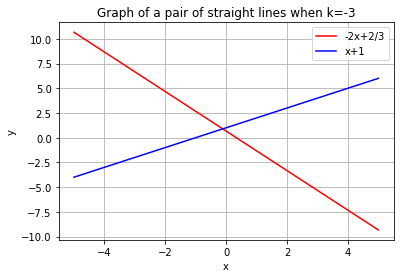
\includegraphics[width=\columnwidth]{solutions/2/6/24/fig1.png}
   \caption{Pair of straight lines when k=-3}
   \label{eq:solutions/2/6/24/fig:1}
\end{figure}
\begin{figure}[!htb]
   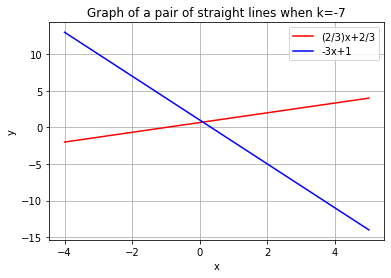
\includegraphics[width=\columnwidth]{solutions/2/6/24/fig2.png}
   \caption{Pair of straight lines when k=-7}
   \label{eq:solutions/2/6/24/fig:2}
\end{figure}
